\chapter{Adaptive Control}
\label{ch:adaptive-control}

\begin{marginfigure}[7mm]
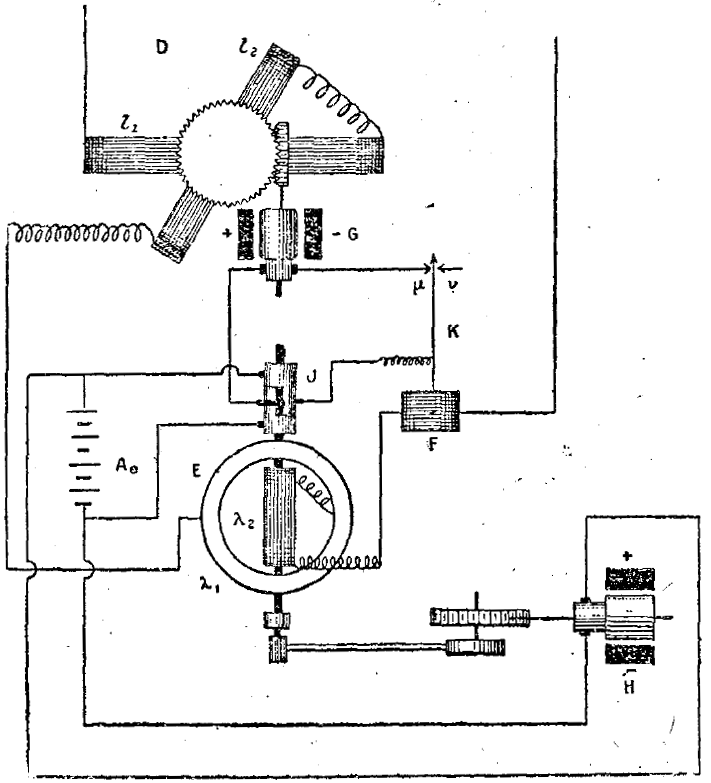
\includegraphics[width=0.9\textwidth]{img/extremum_seeking_controller.png}
\caption[Schematics of one of the first adaptive
controllers.]{Schematics of one of the first adaptive
controllers in the literature, implemented in
hardware.~\citenum{Leblanc:1922:Electrification}}
\label{fig:extremum-seeking-controller}
\end{marginfigure}

\lettrine{C}{ontrollers} that are able to adjust themselves to different
environmental conditions are usually subsumed under the umbrella term
``adaptive control''. Adaptivity is an important concept because there is
always a discrepancy between assumed models and the real world. In fact, for
many control systems a big proportion of development time is spent in
hand-crafting and tuning models. Adaptive control systems aim at learning
models at runtime, or at adjusting them if the environment is changing.

\margincite{Leblanc:1922:Electrification} The idea of adaptive control is quite
old, and many sources (\eg\cite{Ariyur.Krstic:2003:Real}) report the paper by
\citetext{Leblanc:1922:Electrification} as the first paper on this topic, see
Figure~\ref{fig:extremum-seeking-controller} for an illustration of the hardware
implementation. Since then, adaptive controllers have found many applications in
the automatic control of technical systems.

Unfortunately, the term \emph{adaptive control} has no clear definition and the
meaning often depends on the author. For example, in their textbook on
this topic, \textcite{Astrom.Wittenmark:1994:Adaptive} define ``an adaptive
controller [as] a controller with adjustable parameters and a mechanism for
adjusting the parameters''. The definition of adaptive control now depends on
the definition of a parameter, which also is not always clear.

Usually, the states are expected to change more rapidly and as direct response
to control actions and disturbances. Parameters, on the other hand, are
changing more slowly and are therefore seen on a different time
scale.~\cite[\ts3.1]{Filatov.Unbehauen:2004:Adaptive}\iss For example, while
position, velocity and acceleration are usually states, the physical properties
like weight or length of mechanical components are parameters. But also
slowly-varying states like the angle of attack of a plane can be seen as
parameters, since they change slowly, but govern other parts of the overall
dynamics. In hierarchical control systems, the states of a higher level can be
viewed as parameters of a lower one.

\section{Types of Adaptive Controllers}

Typically, adaptive controllers are classified into four different types of
adaptive control schemes
\margincite{Astrom.Wittenmark:1994:Adaptive}%
\margincite{Sastry.Bodson:2011:Adaptive}%
\citenum{Astrom.Wittenmark:1994:Adaptive, Sastry.Bodson:2011:Adaptive}:
\begin{description}
  \item[Gain Scheduling]
  This is the simplest case of an adaptive control system. Based on a
  pre-defined condition (for example, one of the states or parameters being in a
  certain  range), the control system switches between different setpoints or
  operating  conditions. A static feedback control law is provided for every
  setpoint. The  system is adaptive because the local controllers are tuned for
  each setpoint
  individually.~\cite{Leith.Leithead:2000:Survey}
  \item[Model-Reference Adaptive Control] This is a form of extremum seeking
  control, where a performance criterion based on a reference trajectory is
  optimized by parameter tuning. Usually this is done with a gradient-based
  optimization scheme, where the gradients are evaluated by numeric
  differentiation.~\cite{Landau:1974:Survey}
  \item[Self-Tuning Regulators] This is a model-based control strategy. A model
  of the system dynamics is learned or maintained online (\eg via parameter
  tracking in a parametric model). The model of the system is then used to
  calculate a controller with standard model-based control
  techniques.~\cite{Astrom.Wittenmark:1973:Self}
  \item[Dual Control\footnotemark] \footnotetext[1][3mm]{Dual control is
  an integral part of this thesis and will be covered in depth in
  Part~\ref{par:dual-control}.}This is the theoretically ideal way of performing
  adaptive control. An optimal dual controller would perform nonlinear
  stochastic optimal control on a system state that comprises both the states
  and the belief over the system dynamics. This type of controller is of such
  complexity that it is challenging to apply it in
  practice.~\cite{Wittenmark:1995:Adaptive}
\end{description}

Figure~\ref{fig:methods-classification} shows an overview of adaptive control
methods in relation to time of information acquisition.  While all adaptive
control methods are online methods, only dual control takes future measurements
into account.

\begin{figure}%
  \centering
  \inputTikZ{methods_classification}%
  \caption[Classification of adaptive control methods.]{Classification
of adaptive control methods, based on the time of information acquisition
(left to right) and the use of a model (top and bottom).}
  \label{fig:methods-classification}
\end{figure}

Note the distinction between model-free and model-based adaptive controllers.
From the above classifications, \emph{gain scheduling} and
\emph{model-reference adaptive control} are model-free, which means that they
are tuning a control-law\footnote{A control-law is sometimes also called
``policy'', especially in the reinforcement learning community.} directly. The
other two classes, \emph{self-tuning regulators} and \emph{dual control},
qualify as model-based schemes. This means that the model of the process is
adapted and a controller is synthesized from this model according to some
principle.

\section{Model Identification Adaptive Control}

The definition of adaptive control by \textcite{Astrom.Wittenmark:1994:Adaptive}
is relatively broad and can sometimes lead to confusion. Also, the distinction
between adaptive and non-adaptive is much harder to make for model-free
controllers than for model-based ones.\footnote{Essentially all model-free
controllers (except static state-feedback controllers) are adaptive because
they depend on changing parameters. This complicates the discussion quite a
bit.}
In the following, we therefore only consider model-based controllers, where we
assume that the system is governed by a true, but unknown, dynamics function
\begin{equation}
  x_{\tk+1} = f_\tk(x_\tk,u_\tk)
\end{equation}
that depends on the states $x$, the inputs $u$ and the time instance $\tk$. The
adaptive controller builds or updates an estimate $\hat f_\tk$ of the true
dynamics $f_\tk$ and uses it to calculate the control input
\begin{equation}
  u_\tk = c(\hat f_\tk, x_\tk),
\end{equation}
where $c$ is the model-based controller.\footnote{In the case of optimal
control, also a cost function $l_\tk$ would be necessary.}
Consequently, the controllers in this thesis can all be seen as model
identification adaptive controllers in the broader context of adaptive control.

\begin{figure}
  \center%
  \inputTikZ{MIAC_structure}%
  \caption[Structure of a model identification adaptive controller.]{
  Structure of a model identification adaptive controller.
  The estimator maintains a model $\hat f$ of the dynamics which is used by the
  controller together with the state $x$ to generate the control signal $u$.}
\end{figure}

\begin{definition}
  A model identification adaptive controller generates control inputs using
  an continually estimated model of the uncertain and possibly time-varying
  system dynamics.
\end{definition}

Henceforth, we use \emph{adaptive control} as a synonym for \emph{model
identification adaptive control} to simplify reading.

\pagebreak[4]

\section{System Identification and Adaptive Control}

Sometimes there is confusion between system identification
\cite{Ljung:1999:System} (in combination with a regular controller) and adaptive
control. This comes from the fact that both techniques use similar mathematical
methods. The difference lies in the time of information acquisition: While
system identification is done offline and provides a model for a controller,
adaptive control is an online method. While some types of adaptive control even
try to predict the process of information acquisition to the future, all
adaptive methods use the measurements during runtime to adjust the controller
(see also Figure~\ref{fig:methods-classification}).

It is clear that both system identification as well as adaptive control can
``adapt'' to different systems, but while an adaptive controller does the
learning online while controlling, system identification is separate from the
controller. Once the system identification is done, a controller is synthesized
and subsequently used in the control problem. Usually parameters that do not
change between the identification and the use of the control system are
identified with system identification. Other parameters can only be identified
online, either because they are subject to change or because the specific
problem instance can not be identified in advance.

\section{Adaptivity and Robustness}

Adaptivity is not the only way to deal with uncertainties in the model or the
environment. Another possible option is robust control
\cite{Zhou.Doyle:1998:Essentials}. In robust control systems, the controller is
designed to be resilient against uncertainties. This means that deviations in
the nominal parameters and disturbances do not endanger the system's stability.
This is usually done by considering worst case examples and controlling the
system in a way that all worst case examples are still stable.

If a control system is robust to parameter changes, one could argue that
adaptivity is not necessary. But there are still reasons to design adaptive
systems as well. Because robust control systems need to be compatible with
multiple worst case instances of a given problem, in many situations
infeasibility can arise: Not for all scenario distributions or combinations of
worst cases a robust controller does
exist.~\cite{Calafiore.Campi:2006:Scenario}\iss But also when feasibility is
given for the uncertain system, robust control trades performance for worst case
stability. If the control system is adaptive, the performance level can be much
higher after the system is learned because many of the unlikely examples can be
ruled out by the learning process.

Of course, adaptivity and robustness are not exclusive. A robust control system
can be designed relative to the current state of an adaptive control system,
combining the features of both.~\cite{Ioannou.Sun:1996:Robust}
